% Chapter 5: GARCH Seminar - Review Quiz and Practice Exercises
% Beamer Presentation
% Bachelor program, Bucharest University of Economic Studies

\documentclass[9pt, aspectratio=169, t]{beamer}

% Ensure content fits on slides
\setbeamersize{text margin left=8mm, text margin right=8mm}

%=============================================================================
% THEME AND STYLE CONFIGURATION
%=============================================================================
\usetheme{default}
% Using default theme for clean header/footer control

% Color Palette (matching Redispatch PDF)
\definecolor{MainBlue}{RGB}{26, 58, 110}
\definecolor{AccentBlue}{RGB}{26, 58, 110}
\definecolor{IDAred}{RGB}{205, 0, 0}
\definecolor{DarkGray}{RGB}{51, 51, 51}
\definecolor{MediumGray}{RGB}{128, 128, 128}
\definecolor{LightGray}{RGB}{248, 248, 248}
\definecolor{VeryLightGray}{RGB}{235, 235, 235}
\definecolor{KeynoteGray}{RGB}{218, 218, 218}
\definecolor{SectionGray}{RGB}{120, 120, 120}
\definecolor{FooterGray}{RGB}{100, 100, 100}
\definecolor{Crimson}{RGB}{220, 53, 69}
\definecolor{Forest}{RGB}{46, 125, 50}
\definecolor{Amber}{RGB}{181, 133, 63}
\definecolor{Orange}{RGB}{230, 126, 34}
\definecolor{Purple}{RGB}{142, 68, 173}

% Gradient background (exact Keynote 315° gradient: white to RGB 218,218,218)
\setbeamertemplate{background}{%
    \begin{tikzpicture}[remember picture, overlay]
        \shade[shading=axis, shading angle=315,
        top color=white, bottom color=KeynoteGray]
        (current page.south west) rectangle (current page.north east);
    \end{tikzpicture}%
}
% Fallback solid color for compatibility
\setbeamercolor{background canvas}{bg=}

\setbeamercolor{palette primary}{bg=MainBlue, fg=white}
\setbeamercolor{palette secondary}{bg=MainBlue!85, fg=white}
\setbeamercolor{palette tertiary}{bg=MainBlue!70, fg=white}
\setbeamercolor{structure}{fg=MainBlue}
\setbeamercolor{title}{fg=IDAred}
\setbeamercolor{frametitle}{fg=IDAred, bg=}
\setbeamercolor{block title}{bg=MainBlue, fg=white}
\setbeamercolor{block body}{bg=VeryLightGray, fg=DarkGray}
\setbeamercolor{block title alerted}{bg=Crimson, fg=white}
\setbeamercolor{block body alerted}{bg=Crimson!8, fg=DarkGray}
\setbeamercolor{block title example}{bg=Forest, fg=white}
\setbeamercolor{block body example}{bg=Forest!8, fg=DarkGray}
\setbeamercolor{item}{fg=MainBlue}

% Footer colors (override Madrid theme blue)
\setbeamercolor{author in head/foot}{fg=FooterGray, bg=}
\setbeamercolor{title in head/foot}{fg=FooterGray, bg=}
\setbeamercolor{date in head/foot}{fg=FooterGray, bg=}
\setbeamercolor{section in head/foot}{fg=FooterGray, bg=}
\setbeamercolor{subsection in head/foot}{fg=FooterGray, bg=}

% Bullet styles (apply everywhere including blocks)
\setbeamertemplate{itemize item}{\color{MainBlue}$\boxdot$}
\setbeamertemplate{itemize subitem}{\color{MainBlue}$\blacktriangleright$}
\setbeamertemplate{itemize subsubitem}{\color{MainBlue}\tiny$\bullet$}
\setbeamertemplate{itemize/enumerate body begin}{\normalsize}
\setbeamertemplate{itemize/enumerate subbody begin}{\normalsize}

% Item spacing - compact style
\setlength{\leftmargini}{10pt}       % Level 1: minimal indent
\setlength{\leftmarginii}{10pt}      % Level 2: minimal additional indent
% Compact list spacing (zero extra space before/after lists in blocks)
\makeatletter
\def\@listi{\leftmargin\leftmargini \topsep 0pt \parsep 0pt \itemsep 0pt}
\def\@listii{\leftmargin\leftmarginii \topsep 0pt \parsep 0pt \itemsep 0pt}
\makeatother

\setbeamertemplate{navigation symbols}{}

%=============================================================================
% CUSTOM HEADLINE
%=============================================================================
\setbeamertemplate{headline}{%
    \vskip10pt%
    \hbox to \paperwidth{%
        \hskip0.5cm%
        {\small\color{FooterGray}\renewcommand{\hyperlink}[2]{##2}\insertsectionhead}%
        \hfill%
        \textcolor{FooterGray}{\small\insertframenumber}%
        \hskip0.5cm%
    }%
    \vskip4pt%
    {\color{FooterGray}\hrule height 0.4pt}%
}

%=============================================================================
% CUSTOM FOOTER
%=============================================================================
\usepackage{fontawesome5}

\setbeamertemplate{footline}{%
    {\color{FooterGray}\hrule height 0.4pt}%
    \vskip4pt%
    \hbox to \paperwidth{%
        \hskip0.5cm%
        \textcolor{FooterGray}{\small Time Series Analysis and Forecasting}%
        \hfill%
        \raisebox{-0.1em}{%
            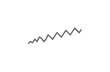
\begin{tikzpicture}[x=0.08em, y=0.08em, line width=0.4pt]
                \draw[FooterGray] (0,3) -- (1,4) -- (2,3.5) -- (3,5) -- (4,4) -- (5,6) -- (6,5.5) -- (7,4) -- (8,5) -- (9,7) -- (10,6) -- (11,5) -- (12,6.5) -- (13,8) -- (14,7) -- (15,6) -- (16,7.5) -- (17,9) -- (18,8) -- (19,7) -- (20,8.5) -- (21,10) -- (22,9) -- (23,8) -- (24,9.5);
            \end{tikzpicture}%
        }%
        \hskip0.5cm%
    }%
    \vskip6pt%
}

%=============================================================================
% PACKAGES
%=============================================================================
\usepackage[utf8]{inputenc}
\usepackage[T1]{fontenc}
\usepackage[english]{babel}
\usepackage{amsmath, amssymb, amsthm}
\usepackage{mathtools}
\usepackage{bm}
\usepackage{tikz}
\usetikzlibrary{arrows.meta, positioning, shapes, calc, decorations.pathreplacing, shadings}
\usepackage{booktabs}
\usepackage{multirow}
\usepackage{array}
\usepackage{graphicx}
\usepackage{hyperref}
\usepackage{colortbl}
\hypersetup{colorlinks=true, linkcolor=MainBlue, urlcolor=MainBlue}
\graphicspath{{../../logos/}{../../charts/}}
\hfuzz=2pt  % Suppress tiny overfull warnings (<2pt)
\vfuzz=2pt  % Suppress tiny vertical overfull warnings (<2pt)

%=============================================================================
% QUANTLET COMMAND
%=============================================================================
\newcommand{\quantlet}[2]{%
    \hfill\href{#2}{%
        \raisebox{-0.15em}{\includegraphics[height=0.7em]{ql_logo.png}}%
        \textcolor{MainBlue}{\tiny\ #1}%
    }%
}

%=============================================================================
% CUSTOM COMMANDS
%=============================================================================
\newcommand{\E}{\mathbb{E}}
\newcommand{\Var}{\text{Var}}
\newcommand{\Cov}{\text{Cov}}
\newcommand{\R}{\mathbb{R}}

%=============================================================================
% TITLE INFORMATION
%=============================================================================
\title[Chapter 5: GARCH Seminar]{Chapter 5: GARCH Seminar}
\subtitle{Review Quiz and Practice Exercises}
\author[Prof. dr. Daniel Traian Pele]{Prof. dr. Daniel Traian Pele\\[0.2cm]\footnotesize\texttt{danpele@ase.ro}}
\institute{Bucharest University of Economic Studies}
\date{Academic Year 2025--2026}

\begin{document}

%=============================================================================
% TITLE SLIDE
%=============================================================================
\begin{frame}[plain]
    \begin{tikzpicture}[remember picture, overlay]
        \fill[IDAred] (current page.north west) rectangle ([yshift=-0.15cm]current page.north east);
        \node[anchor=north west] at ([xshift=0.5cm, yshift=-0.3cm]current page.north west) {
            \href{https://www.ase.ro}{\includegraphics[height=1.1cm]{ase_logo.png}}
        };
        \node[anchor=north] at ([yshift=-0.3cm]current page.north) {
            \href{https://ai4efin.ase.ro}{\includegraphics[height=1.1cm]{ai4efin_logo.png}}
        };
        \node[anchor=north east] at ([xshift=-0.5cm, yshift=-0.3cm]current page.north east) {
            \href{https://www.digital-finance-msca.com}{\includegraphics[height=1.1cm]{msca_logo.png}}
        };
    \end{tikzpicture}
    \vfill
    \begin{center}
        {\Large\textcolor{MediumGray}{Seminar: Volatility Models}}\\[0.3cm]
        {\Huge\textbf{\textcolor{MainBlue}{ARCH, GARCH, EGARCH, TGARCH}}}\\[0.5cm]
        {\Large\textcolor{IDAred}{Review Quiz and Practice Exercises}}
    \end{center}
    \vfill

    \begin{tikzpicture}[remember picture, overlay]
        \fill[IDAred] (current page.south west) rectangle ([yshift=0.15cm]current page.south east);
        \node[anchor=south west] at ([xshift=0.5cm, yshift=0.8cm]current page.south west) {
            \href{https://theida.net}{\includegraphics[height=0.9cm]{ida_logo.png}}
        };
        \node[anchor=south] at ([xshift=-3cm, yshift=0.8cm]current page.south) {
            \href{https://blockchain-research-center.com}{\includegraphics[height=0.9cm]{brc_logo.png}}
        };
        \node[anchor=south] at ([yshift=0.8cm]current page.south) {
            \href{https://quantinar.com}{\includegraphics[height=0.9cm]{qr_logo.png}}
        };
        \node[anchor=south] at ([xshift=3cm, yshift=0.8cm]current page.south) {
            \href{https://quantlet.com}{\includegraphics[height=0.9cm]{ql_logo.png}}
        };
        \node[anchor=south east] at ([xshift=-0.5cm, yshift=0.8cm]current page.south east) {
            \href{https://ipe.ro/new}{\includegraphics[height=0.9cm]{acad_logo.png}}
        };
    \end{tikzpicture}
\end{frame}

%=============================================================================
% TABLE OF CONTENTS
%=============================================================================
\begin{frame}{Seminar Outline}
    \tableofcontents
\end{frame}

%=============================================================================
% SECTION 1: QUIZ
%=============================================================================
\section{Review Quiz}

%-----------------------------------------------------------------------------
% Quiz 1
%-----------------------------------------------------------------------------
\begin{frame}{Question 1}
    \begin{block}{What is ``volatility clustering''?}
        \begin{enumerate}[(A)]
            \item Volatility is constant over time
            \item Periods of high volatility tend to be followed by periods of high volatility
            \item Returns are correlated over time
            \item The return distribution is normal
        \end{enumerate}
    \end{block}

    \vspace{1cm}

    \begin{center}
        \textit{Think about the behavior of financial markets during crisis periods...}
    \end{center}
\end{frame}

\begin{frame}{Answer to Question 1}
    \begin{exampleblock}{Correct Answer: (B)}
        \textbf{Periods of high volatility tend to be followed by periods of high volatility}
    \end{exampleblock}

    \begin{block}{Explanation}
        \begin{itemize}
            \item \textbf{Volatility clustering} is a stylized fact observed in financial time series
            \item ``Turbulent'' periods (with large movements) tend to persist
            \item ``Calm'' periods (with small movements) also tend to persist
            \item This implies that conditional variance $\sigma_t^2$ is \textbf{predictable}
            \item GARCH models capture exactly this phenomenon!
        \end{itemize}
    \end{block}
\end{frame}

%-----------------------------------------------------------------------------
% Quiz 2
%-----------------------------------------------------------------------------
\begin{frame}{Question 2}
    \begin{block}{In the GARCH(1,1) model: $\sigma_t^2 = \omega + \alpha \varepsilon_{t-1}^2 + \beta \sigma_{t-1}^2$}
        What does the parameter $\alpha$ represent?
        \begin{enumerate}[(A)]
            \item Volatility persistence
            \item Baseline volatility level
            \item Reaction to recent shocks (news coefficient)
            \item Unconditional variance
        \end{enumerate}
    \end{block}
\end{frame}

\begin{frame}{Answer to Question 2}
    \begin{exampleblock}{Correct Answer: (C)}
        \textbf{Reaction to recent shocks (news coefficient)}
    \end{exampleblock}

    \begin{block}{Interpretation of GARCH(1,1) Parameters}
        \begin{itemize}
            \item $\omega$ = baseline (floor) volatility level
            \item $\alpha$ = \textbf{reaction} to squared innovations (``news'')
            \item $\beta$ = volatility \textbf{persistence} (memory)
            \item $\alpha + \beta$ = total persistence
        \end{itemize}

        \vspace{0.3cm}
        A large $\alpha$ means volatility reacts strongly to recent shocks.
    \end{block}
\end{frame}

%-----------------------------------------------------------------------------
% Quiz 3
%-----------------------------------------------------------------------------
\begin{frame}{Question 3}
    \begin{block}{What is the stationarity condition for GARCH(1,1)?}
        \begin{enumerate}[(A)]
            \item $\omega > 0$
            \item $\alpha + \beta = 1$
            \item $\alpha + \beta < 1$
            \item $\alpha > \beta$
        \end{enumerate}
    \end{block}
\end{frame}

\begin{frame}{Answer to Question 3}
    \begin{exampleblock}{Correct Answer: (C)}
        \textbf{$\alpha + \beta < 1$}
    \end{exampleblock}

    \begin{block}{Complete Conditions}
        For GARCH(1,1) stationarity:
        \begin{itemize}
            \item $\omega > 0$ (ensures positive variance)
            \item $\alpha \geq 0$, $\beta \geq 0$ (non-negativity)
            \item $\alpha + \beta < 1$ (\textbf{strict stationarity})
        \end{itemize}

        \vspace{0.3cm}
        If $\alpha + \beta = 1$ $\Rightarrow$ IGARCH (shocks have permanent effect)
    \end{block}
\end{frame}

%-----------------------------------------------------------------------------
% Quiz 4
%-----------------------------------------------------------------------------
\begin{frame}{Question 4}
    \begin{block}{What is the formula for unconditional variance in GARCH(1,1)?}
        \begin{enumerate}[(A)]
            \item $\bar{\sigma}^2 = \omega$
            \item $\bar{\sigma}^2 = \dfrac{\omega}{1 - \alpha}$
            \item $\bar{\sigma}^2 = \dfrac{\omega}{1 - \alpha - \beta}$
            \item $\bar{\sigma}^2 = \dfrac{\omega}{\alpha + \beta}$
        \end{enumerate}
    \end{block}
\end{frame}

\begin{frame}{Answer to Question 4}
    \begin{exampleblock}{Correct Answer: (C)}
        $\bar{\sigma}^2 = \dfrac{\omega}{1 - \alpha - \beta}$
    \end{exampleblock}

    \begin{block}{Derivation}
        Taking unconditional expectation of GARCH(1,1):
        \begin{align*}
            \E[\sigma_t^2] &= \omega + \alpha \E[\varepsilon_{t-1}^2] + \beta \E[\sigma_{t-1}^2] \\
            \bar{\sigma}^2 &= \omega + \alpha \bar{\sigma}^2 + \beta \bar{\sigma}^2 \\
            \bar{\sigma}^2 (1 - \alpha - \beta) &= \omega \\
            \bar{\sigma}^2 &= \frac{\omega}{1 - \alpha - \beta}
        \end{align*}
    \end{block}
\end{frame}

%-----------------------------------------------------------------------------
% Quiz 5
%-----------------------------------------------------------------------------
\begin{frame}{Question 5}
    \begin{block}{What is the ``leverage effect''?}
        \begin{enumerate}[(A)]
            \item Positive shocks increase volatility more than negative shocks
            \item Negative shocks increase volatility more than positive shocks
            \item Volatility is independent of shock sign
            \item Returns are asymmetric
        \end{enumerate}
    \end{block}
\end{frame}

\begin{frame}{Answer to Question 5}
    \begin{exampleblock}{Correct Answer: (B)}
        \textbf{Negative shocks increase volatility more than positive shocks}
    \end{exampleblock}

    \begin{block}{Explanation}
        \begin{itemize}
            \item Empirically observed in stock markets
            \item When prices fall, firm leverage increases (debt becomes larger relative to equity)
            \item This makes the firm riskier $\Rightarrow$ higher volatility
            \item Standard GARCH \textbf{cannot} capture this effect (depends on $\varepsilon^2$)
            \item Solutions: \textbf{EGARCH}, \textbf{GJR-GARCH}, \textbf{TGARCH}
        \end{itemize}
    \end{block}
\end{frame}

%-----------------------------------------------------------------------------
% Quiz 6
%-----------------------------------------------------------------------------
\begin{frame}{Question 6}
    \begin{block}{In the EGARCH model, a negative $\gamma$ parameter indicates:}
        \begin{enumerate}[(A)]
            \item Absence of leverage effect
            \item Presence of leverage effect
            \item Constant volatility
            \item Non-stationary model
        \end{enumerate}
    \end{block}
\end{frame}

\begin{frame}{Answer to Question 6}
    \begin{exampleblock}{Correct Answer: (B)}
        \textbf{Presence of leverage effect}
    \end{exampleblock}

    \begin{block}{EGARCH(1,1)}
        \[
            \ln(\sigma_t^2) = \omega + \alpha (|z_{t-1}| - \E[|z|]) + \gamma z_{t-1} + \beta \ln(\sigma_{t-1}^2)
        \]

        \begin{itemize}
            \item $\gamma < 0$: negative shock ($z < 0$) $\Rightarrow$ increases $\ln(\sigma_t^2)$
            \item $\gamma > 0$: inverse effect (less common)
            \item $\gamma = 0$: symmetric effect (like GARCH)
        \end{itemize}
    \end{block}
\end{frame}

%-----------------------------------------------------------------------------
% Quiz 7
%-----------------------------------------------------------------------------
\begin{frame}{Question 7}
    \begin{block}{What is the main advantage of EGARCH over GARCH?}
        \begin{enumerate}[(A)]
            \item Faster to estimate
            \item No non-negativity constraints needed
            \item Fewer parameters
            \item Easier to interpret
        \end{enumerate}
    \end{block}
\end{frame}

\begin{frame}{Answer to Question 7}
    \begin{exampleblock}{Correct Answer: (B)}
        \textbf{No non-negativity constraints needed}
    \end{exampleblock}

    \begin{block}{EGARCH Advantages}
        \begin{itemize}
            \item Models $\ln(\sigma_t^2)$, not $\sigma_t^2$
            \item $\sigma_t^2 = e^{\ln(\sigma_t^2)} > 0$ \textbf{automatically}, regardless of parameter values
            \item GARCH requires $\omega > 0$, $\alpha \geq 0$, $\beta \geq 0$
            \item During estimation, these constraints can cause convergence problems
        \end{itemize}
    \end{block}
\end{frame}

%-----------------------------------------------------------------------------
% Quiz 8
%-----------------------------------------------------------------------------
\begin{frame}{Question 8}
    \begin{block}{Which test do we use to detect ARCH effects in residuals?}
        \begin{enumerate}[(A)]
            \item Dickey-Fuller test
            \item Ljung-Box test on residuals
            \item Engle's ARCH-LM test
            \item Breusch-Pagan test
        \end{enumerate}
    \end{block}
\end{frame}

\begin{frame}{Answer to Question 8}
    \begin{exampleblock}{Correct Answer: (C)}
        \textbf{Engle's ARCH-LM test}
    \end{exampleblock}

    \begin{block}{ARCH-LM Test Procedure}
        \begin{enumerate}
            \item Estimate mean model, obtain residuals $\hat{\varepsilon}_t$
            \item Compute $\hat{\varepsilon}_t^2$
            \item Regress: $\hat{\varepsilon}_t^2 = \beta_0 + \beta_1 \hat{\varepsilon}_{t-1}^2 + \cdots + \beta_q \hat{\varepsilon}_{t-q}^2 + u_t$
            \item Test statistic: $LM = T \cdot R^2 \sim \chi^2(q)$ under $H_0$
        \end{enumerate}

        $H_0$: No ARCH effects $\quad$ $H_1$: ARCH effects present
    \end{block}
\end{frame}

%-----------------------------------------------------------------------------
% Quiz 9
%-----------------------------------------------------------------------------
\begin{frame}{Question 9}
    \begin{block}{For S\&P 500, typical values of $\alpha + \beta$ in GARCH(1,1) are:}
        \begin{enumerate}[(A)]
            \item 0.50 -- 0.70
            \item 0.70 -- 0.85
            \item 0.95 -- 0.99
            \item Greater than 1
        \end{enumerate}
    \end{block}
\end{frame}

\begin{frame}{Answer to Question 9}
    \begin{exampleblock}{Correct Answer: (C)}
        \textbf{0.95 -- 0.99}
    \end{exampleblock}

    \begin{block}{Highly Persistent Volatility}
        \begin{itemize}
            \item Financial time series exhibit very persistent volatility
            \item $\alpha + \beta \approx 0.98$ for S\&P 500
            \item Half-life: $HL = \frac{\ln(0.5)}{\ln(\alpha + \beta)} \approx 35-60$ days
            \item This means a volatility shock dissipates over several months
        \end{itemize}

        \vspace{0.3cm}
        \begin{center}
            \begin{tabular}{lc}
                \toprule
                \textbf{Series} & $\bm{\alpha + \beta}$ \\
                \midrule
                S\&P 500 & 0.97--0.99 \\
                Bitcoin & 0.90--0.98 \\
                EUR/USD & 0.96--0.99 \\
                \bottomrule
            \end{tabular}
        \end{center}
    \end{block}
\end{frame}

%-----------------------------------------------------------------------------
% Quiz 10
%-----------------------------------------------------------------------------
\begin{frame}{Question 10}
    \begin{block}{Which distribution is most commonly used for GARCH innovations to capture fat tails?}
        \begin{enumerate}[(A)]
            \item Normal
            \item Uniform
            \item Student-t
            \item Exponential
        \end{enumerate}
    \end{block}
\end{frame}

\begin{frame}{Answer to Question 10}
    \begin{exampleblock}{Correct Answer: (C)}
        \textbf{Student-t}
    \end{exampleblock}

    \begin{block}{Innovation Distributions}
        \begin{itemize}
            \item \textbf{Normal}: standard, but underestimates extreme risk
            \item \textbf{Student-t}: fat tails, parameter $\nu$ (degrees of freedom)
            \item \textbf{GED}: Generalized Error Distribution, flexible
            \item \textbf{Skewed Student-t}: asymmetry + fat tails
        \end{itemize}

        \vspace{0.3cm}
        For S\&P 500: $\nu \approx 5-8$ (significantly fatter tails than normal)
    \end{block}
\end{frame}

%=============================================================================
% SECTION 2: TRUE/FALSE
%=============================================================================
\section{True/False Questions}

\begin{frame}{True or False?}
    \begin{enumerate}
        \item ARIMA models can capture volatility clustering.

        \vspace{0.3cm}

        \item In GARCH(1,1), if $\alpha + \beta = 1$, the model is called IGARCH.

        \vspace{0.3cm}

        \item GJR-GARCH uses an indicator variable for negative shocks.

        \vspace{0.3cm}

        \item GARCH volatility forecasts converge to zero in the long run.

        \vspace{0.3cm}

        \item EGARCH can have negative parameters without generating negative variance.

        \vspace{0.3cm}

        \item Value at Risk (VaR) can be calculated using GARCH volatility forecasts.
    \end{enumerate}
\end{frame}

\begin{frame}{True/False Answers}
    \begin{enumerate}
        \item \textbf{FALSE} --- ARIMA assumes constant variance; GARCH models volatility.

        \vspace{0.2cm}

        \item \textbf{TRUE} --- IGARCH = Integrated GARCH, volatility has unit root.

        \vspace{0.2cm}

        \item \textbf{TRUE} --- $I_{t-1} = 1$ if $\varepsilon_{t-1} < 0$, else 0.

        \vspace{0.2cm}

        \item \textbf{FALSE} --- Converges to unconditional variance $\bar{\sigma}^2$, not zero.

        \vspace{0.2cm}

        \item \textbf{TRUE} --- Models $\ln(\sigma_t^2)$, so $\sigma_t^2 = e^{\ln(\sigma_t^2)} > 0$ always.

        \vspace{0.2cm}

        \item \textbf{TRUE} --- $\text{VaR}_\alpha = z_\alpha \cdot \sigma_{t+1}$ (for zero mean).
    \end{enumerate}
\end{frame}

%=============================================================================
% SECTION 3: PRACTICE PROBLEMS
%=============================================================================
\section{Practice Problems}

\begin{frame}{Problem 1: Calculating Unconditional Variance}
    \begin{block}{Statement}
        A GARCH(1,1) model has estimated parameters:
        \begin{itemize}
            \item $\omega = 0.000002$
            \item $\alpha = 0.08$
            \item $\beta = 0.90$
        \end{itemize}

        \vspace{0.3cm}
        Calculate:
        \begin{enumerate}[(a)]
            \item Daily unconditional variance
            \item Daily unconditional volatility (as percentage)
            \item Annualized volatility (assuming 252 trading days)
            \item Volatility half-life
        \end{enumerate}
    \end{block}
\end{frame}

\begin{frame}{Solution to Problem 1}
    \begin{exampleblock}{Answers}
        \begin{enumerate}[(a)]
            \item $\bar{\sigma}^2 = \dfrac{\omega}{1 - \alpha - \beta} = \dfrac{0.000002}{1 - 0.08 - 0.90} = \dfrac{0.000002}{0.02} = 0.0001$

            \vspace{0.2cm}

            \item $\bar{\sigma} = \sqrt{0.0001} = 0.01 = 1\%$ per day

            \vspace{0.2cm}

            \item $\sigma_{\text{annual}} = \bar{\sigma} \times \sqrt{252} = 0.01 \times 15.87 = 15.87\%$ per year

            \vspace{0.2cm}

            \item $HL = \dfrac{\ln(0.5)}{\ln(\alpha + \beta)} = \dfrac{\ln(0.5)}{\ln(0.98)} = \dfrac{-0.693}{-0.0202} \approx 34$ days
        \end{enumerate}
    \end{exampleblock}

    \begin{block}{Interpretation}
        Volatility of 15.87\% per year is typical for a stock index. Half-life of 34 days means a volatility shock is reduced by half after about 7 weeks.
    \end{block}
\end{frame}

\begin{frame}{Problem 2: Volatility Forecast}
    \begin{block}{Statement}
        Using the GARCH(1,1) model from Problem 1:
        \begin{itemize}
            \item $\omega = 0.000002$, $\alpha = 0.08$, $\beta = 0.90$
            \item At time $T$: $\varepsilon_T = -0.03$ (3\% drop), $\sigma_T^2 = 0.0004$
        \end{itemize}

        \vspace{0.3cm}
        Calculate volatility forecasts for:
        \begin{enumerate}[(a)]
            \item $\sigma_{T+1}^2$ (one step ahead)
            \item $\sigma_{T+5}^2$ (five steps ahead)
            \item $\sigma_{T+100}^2$ (one hundred steps ahead)
        \end{enumerate}
    \end{block}
\end{frame}

\begin{frame}{Solution to Problem 2}
    \begin{exampleblock}{Answers}
        \begin{enumerate}[(a)]
            \item $\sigma_{T+1}^2 = \omega + \alpha \varepsilon_T^2 + \beta \sigma_T^2$
            \[
                = 0.000002 + 0.08 \times (0.03)^2 + 0.90 \times 0.0004 = 0.000434
            \]
            Volatility: $\sqrt{0.000434} = 2.08\%$

            \vspace{0.2cm}

            \item $\E_T[\sigma_{T+5}^2] = \bar{\sigma}^2 + (0.98)^4 (\sigma_{T+1}^2 - \bar{\sigma}^2)$
            \[
                = 0.0001 + 0.922 \times (0.000434 - 0.0001) = 0.000408
            \]
            Volatility: $\sqrt{0.000408} = 2.02\%$

            \vspace{0.2cm}

            \item $\E_T[\sigma_{T+100}^2] = 0.0001 + (0.98)^{99} \times 0.000334 \approx 0.000145$

            Volatility: $\sqrt{0.000145} = 1.20\%$ (close to $\bar{\sigma} = 1\%$)
        \end{enumerate}
    \end{exampleblock}
\end{frame}

\begin{frame}{Problem 3: Value at Risk}
    \begin{block}{Statement}
        A portfolio of 1,000,000 EUR is invested in stocks with returns modeled by GARCH(1,1).

        Tomorrow's volatility forecast: $\sigma_{T+1} = 2\%$ daily.

        Assuming normally distributed returns with zero mean, calculate:
        \begin{enumerate}[(a)]
            \item VaR at 95\% (1 day)
            \item VaR at 99\% (1 day)
            \item VaR at 99\% (10 days), using ``square root of time'' rule
        \end{enumerate}

        \vspace{0.3cm}
        Quantiles: $z_{0.05} = 1.645$, $z_{0.01} = 2.326$
    \end{block}
\end{frame}

\begin{frame}{Solution to Problem 3}
    \begin{exampleblock}{Answers}
        \begin{enumerate}[(a)]
            \item VaR 95\% (1 day):
            \[
                \text{VaR}_{95\%} = 1.645 \times 0.02 \times 1{,}000{,}000 = 32{,}900 \text{ EUR}
            \]

            \vspace{0.2cm}

            \item VaR 99\% (1 day):
            \[
                \text{VaR}_{99\%} = 2.326 \times 0.02 \times 1{,}000{,}000 = 46{,}520 \text{ EUR}
            \]

            \vspace{0.2cm}

            \item VaR 99\% (10 days):
            \[
                \text{VaR}_{99\%, 10d} = \text{VaR}_{99\%, 1d} \times \sqrt{10} = 46{,}520 \times 3.162 = 147{,}100 \text{ EUR}
            \]
        \end{enumerate}
    \end{exampleblock}

    \begin{alertblock}{Caution}
        In practice, for Student-t distribution, quantiles are larger (fatter tails)!
    \end{alertblock}
\end{frame}

\begin{frame}{Problem 4: Model Identification}
    \begin{block}{Statement}
        Analyze the following estimation results and identify the model:

        \vspace{0.3cm}
        \begin{center}
            \begin{tabular}{lcc}
                \toprule
                \textbf{Parameter} & \textbf{Estimate} & \textbf{Std. Error} \\
                \midrule
                $\omega$ & 0.0000015 & 0.0000005 \\
                $\alpha$ & 0.0550 & 0.0120 \\
                $\gamma$ & 0.0850 & 0.0180 \\
                $\beta$ & 0.9100 & 0.0150 \\
                \bottomrule
            \end{tabular}
        \end{center}

        \vspace{0.3cm}
        \begin{enumerate}[(a)]
            \item What model is this?
            \item Is leverage effect present?
            \item What is the impact of negative vs positive shocks?
            \item Is the model stationary?
        \end{enumerate}
    \end{block}
\end{frame}

\begin{frame}{Solution to Problem 4}
    \begin{exampleblock}{Answers}
        \begin{enumerate}[(a)]
            \item \textbf{GJR-GARCH(1,1,1)} --- presence of $\gamma$ parameter (threshold/asymmetry)

            \vspace{0.2cm}

            \item \textbf{Yes, leverage effect present}: $\gamma = 0.085 > 0$ and significant

            \vspace{0.2cm}

            \item Impact:
            \begin{itemize}
                \item Positive shock: impact = $\alpha = 0.055$
                \item Negative shock: impact = $\alpha + \gamma = 0.055 + 0.085 = 0.140$
                \item Negative shocks have \textbf{2.5x greater} impact!
            \end{itemize}

            \vspace{0.2cm}

            \item Stationarity: $\alpha + \gamma/2 + \beta = 0.055 + 0.0425 + 0.91 = 1.0075$

            \textbf{On the edge!} Almost IGARCH. Very persistent model.
        \end{enumerate}
    \end{exampleblock}
\end{frame}

%=============================================================================
% SECTION 4: PYTHON WORKFLOW
%=============================================================================
\section{Python Workflow}

\begin{frame}[fragile]{Step 1: Load and Prepare Data}
\begin{verbatim}
import pandas as pd
import numpy as np
import yfinance as yf
from arch import arch_model
from arch.unitroot import ADF

# Download S&P 500 data
data = yf.download('^GSPC', start='2010-01-01', end='2024-01-01')
returns = 100 * data['Adj Close'].pct_change().dropna()

# Check stationarity
adf = ADF(returns)
print(f'ADF statistic: {adf.stat:.4f}')
print(f'p-value: {adf.pvalue:.4f}')
\end{verbatim}
\end{frame}

\begin{frame}[fragile]{Step 2: Test for ARCH Effects}
\begin{verbatim}
from statsmodels.stats.diagnostic import het_arch

# ARCH-LM test on residuals
residuals = returns - returns.mean()
lm_stat, lm_pvalue, f_stat, f_pvalue = het_arch(residuals, nlags=10)

print(f'ARCH-LM statistic: {lm_stat:.4f}')
print(f'p-value: {lm_pvalue:.4f}')

if lm_pvalue < 0.05:
    print('=> ARCH effects present! GARCH modeling justified.')
\end{verbatim}
\end{frame}

\begin{frame}[fragile]{Step 3: Estimate Models}
\begin{verbatim}
# GARCH(1,1) with Student-t distribution
model_garch = arch_model(returns, vol='Garch', p=1, q=1, dist='t')
res_garch = model_garch.fit(disp='off')
print(res_garch.summary())

# GJR-GARCH(1,1,1)
model_gjr = arch_model(returns, vol='Garch', p=1, o=1, q=1, dist='t')
res_gjr = model_gjr.fit(disp='off')

# EGARCH(1,1)
model_egarch = arch_model(returns, vol='EGARCH', p=1, q=1, dist='t')
res_egarch = model_egarch.fit(disp='off')

# Compare AIC
print(f'GARCH AIC: {res_garch.aic:.2f}')
print(f'GJR AIC: {res_gjr.aic:.2f}')
print(f'EGARCH AIC: {res_egarch.aic:.2f}')
\end{verbatim}
\end{frame}

\begin{frame}[fragile]{Step 4: Diagnostics}
\begin{verbatim}
# Standardized residuals
std_resid = res_gjr.std_resid

# Ljung-Box test on squared residuals
from statsmodels.stats.diagnostic import acorr_ljungbox
lb_test = acorr_ljungbox(std_resid**2, lags=10, return_df=True)
print(lb_test)

# Check for remaining ARCH effects
lm_stat2, lm_pval2, _, _ = het_arch(std_resid, nlags=5)
print(f'ARCH-LM residuals: stat={lm_stat2:.2f}, p={lm_pval2:.4f}')

if lm_pval2 > 0.05:
    print('=> No remaining ARCH effects. Model OK!')
\end{verbatim}
\end{frame}

\begin{frame}[fragile]{Step 5: Forecast and VaR}
\begin{verbatim}
# Forecast 10 days ahead
forecasts = res_gjr.forecast(horizon=10)
vol_forecast = np.sqrt(forecasts.variance.values[-1, :])

print('Volatility forecast (%):', vol_forecast)

# Value at Risk 99%
portfolio_value = 1_000_000
VaR_99 = 2.326 * vol_forecast[0] / 100 * portfolio_value
print(f'VaR 99% (1 day): {VaR_99:,.0f} EUR')

# 10-day VaR
VaR_99_10d = VaR_99 * np.sqrt(10)
print(f'VaR 99% (10 days): {VaR_99_10d:,.0f} EUR')
\end{verbatim}
\end{frame}

%=============================================================================
% SECTION 5: SUMMARY
%=============================================================================
\section{Summary}

\begin{frame}{Seminar Summary}
    \begin{block}{Key Concepts}
        \begin{itemize}
            \item \textbf{ARCH}: conditional variance depends on past shocks
            \item \textbf{GARCH}: adds persistence through lagged variance
            \item \textbf{EGARCH/GJR}: capture leverage effect (asymmetry)
            \item \textbf{Stationarity}: $\alpha + \beta < 1$
        \end{itemize}
    \end{block}

    \begin{block}{Important Formulas}
        \begin{itemize}
            \item Unconditional variance: $\bar{\sigma}^2 = \frac{\omega}{1 - \alpha - \beta}$
            \item Half-life: $HL = \frac{\ln(0.5)}{\ln(\alpha + \beta)}$
            \item VaR: $\text{VaR}_\alpha = z_\alpha \cdot \sigma \cdot V$
        \end{itemize}
    \end{block}

    \begin{alertblock}{Practical Tip}
        Use Student-t distribution to capture fat tails. Verify absence of ARCH effects in residuals!
    \end{alertblock}
\end{frame}

\begin{frame}{Homework Exercises}
    \begin{block}{Exercise 1}
        Download daily returns for BET (BVB index) and estimate a GARCH(1,1) model. Compare persistence ($\alpha + \beta$) with S\&P 500.
    \end{block}

    \begin{block}{Exercise 2}
        For Bitcoin, estimate GARCH, EGARCH, and GJR-GARCH. Is leverage effect present for cryptocurrencies?
    \end{block}

    \begin{block}{Exercise 3}
        Calculate daily VaR for a portfolio of 100,000 EUR invested in EUR/USD, using GARCH-forecasted volatility.
    \end{block}

    \begin{block}{Exercise 4}
        Compare GARCH(1,1) volatility forecast with realized volatility (sum of squared returns) for a 20-day period.
    \end{block}
\end{frame}

\end{document}
